% Options for packages loaded elsewhere
\PassOptionsToPackage{unicode}{hyperref}
\PassOptionsToPackage{hyphens}{url}
%
\documentclass[
]{scrreprt}
\usepackage{amsmath,amssymb}
\usepackage{iftex}
\ifPDFTeX
  \usepackage[T1]{fontenc}
  \usepackage[utf8]{inputenc}
  \usepackage{textcomp} % provide euro and other symbols
\else % if luatex or xetex
  \usepackage{unicode-math} % this also loads fontspec
  \defaultfontfeatures{Scale=MatchLowercase}
  \defaultfontfeatures[\rmfamily]{Ligatures=TeX,Scale=1}
\fi
\usepackage{lmodern}
\ifPDFTeX\else
  % xetex/luatex font selection
\fi
% Use upquote if available, for straight quotes in verbatim environments
\IfFileExists{upquote.sty}{\usepackage{upquote}}{}
\IfFileExists{microtype.sty}{% use microtype if available
  \usepackage[]{microtype}
  \UseMicrotypeSet[protrusion]{basicmath} % disable protrusion for tt fonts
}{}
\makeatletter
\@ifundefined{KOMAClassName}{% if non-KOMA class
  \IfFileExists{parskip.sty}{%
    \usepackage{parskip}
  }{% else
    \setlength{\parindent}{0pt}
    \setlength{\parskip}{6pt plus 2pt minus 1pt}}
}{% if KOMA class
  \KOMAoptions{parskip=half}}
\makeatother
\usepackage{xcolor}
\usepackage{longtable,booktabs,array}
\usepackage{calc} % for calculating minipage widths
% Correct order of tables after \paragraph or \subparagraph
\usepackage{etoolbox}
\makeatletter
\patchcmd\longtable{\par}{\if@noskipsec\mbox{}\fi\par}{}{}
\makeatother
% Allow footnotes in longtable head/foot
\IfFileExists{footnotehyper.sty}{\usepackage{footnotehyper}}{\usepackage{footnote}}
\makesavenoteenv{longtable}
\usepackage{graphicx}
\makeatletter
\def\maxwidth{\ifdim\Gin@nat@width>\linewidth\linewidth\else\Gin@nat@width\fi}
\def\maxheight{\ifdim\Gin@nat@height>\textheight\textheight\else\Gin@nat@height\fi}
\makeatother
% Scale images if necessary, so that they will not overflow the page
% margins by default, and it is still possible to overwrite the defaults
% using explicit options in \includegraphics[width, height, ...]{}
\setkeys{Gin}{width=\maxwidth,height=\maxheight,keepaspectratio}
% Set default figure placement to htbp
\makeatletter
\def\fps@figure{htbp}
\makeatother
\usepackage{soul}
\setlength{\emergencystretch}{3em} % prevent overfull lines
\providecommand{\tightlist}{%
  \setlength{\itemsep}{0pt}\setlength{\parskip}{0pt}}
\setcounter{secnumdepth}{5}
\ifLuaTeX
\usepackage[bidi=basic]{babel}
\else
\usepackage[bidi=default]{babel}
\fi
\babelprovide[main,import]{dutch}
% get rid of language-specific shorthands (see #6817):
\let\LanguageShortHands\languageshorthands
\def\languageshorthands#1{}
\ifLuaTeX
  \usepackage{selnolig}  % disable illegal ligatures
\fi
\IfFileExists{bookmark.sty}{\usepackage{bookmark}}{\usepackage{hyperref}}
\IfFileExists{xurl.sty}{\usepackage{xurl}}{} % add URL line breaks if available
\urlstyle{same}
\hypersetup{
  pdftitle={Bemonstering waterkolom oppervlaktewater},
  pdflang={nl},
  hidelinks,
  pdfcreator={LaTeX via pandoc}}

\title{Bemonstering waterkolom oppervlaktewater}
\usepackage{orcidlink}

\author{Scheers, Kevin\,\orcidlink{0000-0002-4756-4247}}

\date{2021-02-17}

\begin{document}

\maketitle

{
\setcounter{tocdepth}{1}
\tableofcontents
}
\chapter*{Metadata}\label{metadata}
\addcontentsline{toc}{chapter}{Metadata}

\begin{longtable}[]{@{}
  >{\raggedright\arraybackslash}p{(\columnwidth - 10\tabcolsep) * \real{0.3229}}
  >{\raggedright\arraybackslash}p{(\columnwidth - 10\tabcolsep) * \real{0.2083}}
  >{\raggedright\arraybackslash}p{(\columnwidth - 10\tabcolsep) * \real{0.1562}}
  >{\raggedright\arraybackslash}p{(\columnwidth - 10\tabcolsep) * \real{0.1562}}
  >{\raggedright\arraybackslash}p{(\columnwidth - 10\tabcolsep) * \real{0.0729}}
  >{\raggedright\arraybackslash}p{(\columnwidth - 10\tabcolsep) * \real{0.0833}}@{}}
\toprule\noalign{}
\begin{minipage}[b]{\linewidth}\raggedright
reviewers
\end{minipage} & \begin{minipage}[b]{\linewidth}\raggedright
documentbeheerder
\end{minipage} & \begin{minipage}[b]{\linewidth}\raggedright
protocolcode
\end{minipage} & \begin{minipage}[b]{\linewidth}\raggedright
versienummer
\end{minipage} & \begin{minipage}[b]{\linewidth}\raggedright
taal
\end{minipage} & \begin{minipage}[b]{\linewidth}\raggedright
thema
\end{minipage} \\
\midrule\noalign{}
\endhead
\bottomrule\noalign{}
\endlastfoot
An Leyssen, Luc Denys, Geert
De Knijf, Toon Westra & Toon Westra & sfp-114-nl & 2024.04 & nl & water \\
\end{longtable}

Controleer \href{../standard-field-protocols-sfp.html}{deze tabel} om te zien of een meer recente versie beschikbaar is.

\chapter{Wijzigingen t.o.v. vorige versies}\label{wijzigingen-t.o.v.-vorige-versies}

\section{\texorpdfstring{\href{../2024.04/index.html}{2024.04}}{2024.04}}\label{section}

\chapter{Afhankelijkheden}\label{afhankelijkheden}

Procedures waarnaar in deze procedure verwezen wordt:

\begin{itemize}
\item
  SOP-005: Richtlijnen voor conserveren van watermonsters, chemische variabelen en praktische handelingen op terrein
\item
  SVP-015: Bioveiligheidsmaatregelen (in opmaak)
\item
  SVP-112: Veiligheid in en rond water (in opmaak)
\end{itemize}

Procedures die verwijzen naar deze procedure:

\begin{itemize}
\item
  SPP-116: Abiotische staalname stilstaande wateren
\item
  SPP-117: Abiotische staalname stromende wateren
\item
  SVP-115: Veldmeting abiotiek oppervlaktewater met behulp van WTW Multi 3430 veldmeter
\end{itemize}

\chapter{Onderwerp}\label{onderwerp}

\section{Definities en afkortingen}\label{definities-en-afkortingen}

Hieronder worden enkele vaktechnische termen en afkortingen gedefinieerd.

\textbf{ICP:} inductief gekoppeld plasma, een analytische analyse waarbij chemische elementen en met name metalen in een staal bepaald worden door dit in een plasma te brengen en vervolgens het geëmitteerde licht te analyseren.

\textbf{Mengstaal:} een staal bekomen door het mengen van meerdere deelstalen. De deelstalen worden op verschillende, doorgaans ruimtelijk gespreide, plaatsen binnen eenzelfde staalnamelocatie genomen.

\textbf{Oppervlaktewater:} al het permanent of op geregelde tijdstippen stilstaande of stromende water op het landoppervlak, aan de landzijde van de basislijn vanaf waar de breedte van de territoriale zee wordt gemeten (DIW 2003).

\textbf{PVI:} `plant volume infested', ook wel `percent volume infested' of `percent volume inhabited' (Canfield et al.~1984); het percentage van het watervolume dat ingenomen wordt door ondergedoken vegetatie.

\textbf{Sapropelium:} rottingsslib; afzetting van organisch sediment in anaerobe omstandigheden.

\textbf{Staal of monster:} Een portie die geselecteerd wordt uit een grotere hoeveelheid. In dit protocol bestaat het staal steeds uit een hoeveelheid water van de staalnamelocatie (poel, vijver, plas, \ldots).

\textbf{Staalnamelocatie} of \textbf{steekproefeenheid}: het waterlichaam (poel, vijver, \ldots) waarvan de abiotische karakterisatie wordt beoogd en waarbinnen het staalnamepunt zich bevind. Voor stilstaande wateren is dit het gehele waterlichaam, voor waterlopen is dit een 100 meter segment van de waterloop (dit segment wordt aangeduid als het meest stroomafwaarts gelegen punt van het te bemonsteren 100 meter segment).

\textbf{Staalnamepunt:} de exacte plaats binnen de staalnamelocatie waar de abiotische staalname wordt uitgevoerd.

\textbf{Waterbodem:} bodemsubstraat dat zich onder de waterkolom bevindt, inclusief slib en sapropelium.

\textbf{Waterkolom:} de diepte van het water van de waterspiegel (het wateroppervlak) tot de onderwaterbodem.

\section{Doelstelling en toepassingsgebied}\label{doelstelling-en-toepassingsgebied}

Dit protocol beschrijft een methode voor het nemen van een waterstaal als schepstaal met een maatbeker en staalname-emmer in oppervlaktewater voor analyse van de watersamenstelling. Dit staal is enkel representatief voor de watersamenstelling nabij de oppervlakte. Het staal wordt vervolgens geanalyseerd in een analytisch laboratorium, met als doel de fysisch-chemische toestand van het oppervlaktewater op een specifieke plaats en tijdstip te bepalen, maar kan ook gebruikt worden om ter plaatse door middel van apparatuur of testkits bepaalde kenmerken onmiddellijk te bepalen. Voor een representatief beeld van de fysisch-chemische toestand is het doorgaans nodig om de staalname en metingen meermaals in de tijd te herhalen. In dit document behandelen we het veldmateriaal, de werkwijze, de randvoorwaarden, veiligheidsnormen en andere richtlijnen voor de staalname, het transport en de voorbereiding van waterstalen voor verdere analyse in het laboratorium. De beschreven methode is specifiek gericht op oppervlaktewater en is dus niet bedoeld voor grondwater of kustwateren.

\chapter{Beperkingen van het protocol}\label{beperkingen-van-het-protocol}

In bepaalde omstandigheden, vooral ten gevolge van specifieke weersomstandigheden, kan het protocol niet (volledig) gevolgd worden. Bij onweer met (kans op-) blikseminslag kan de veiligheid van de staalnemer niet worden gegarandeerd. Bij vriestemperaturen kan de staalnamelocatie bedekt zijn door een dikke laag ijs, of kan de waterkolom geheel bevroren zijn, zodat het onmogelijk, of niet wenselijk is om een staal te nemen. Ook als er geen of zeer weinig water boven de waterbodem aanwezig is, is een staalname niet, of niet op de voorgeschreven manier, mogelijk. Wanneer er geen staal kan genomen worden, wordt dit steeds vermeld op het staalnameformulier in het opmerkingenveld met vermelding van de reden.

Een zeer lage waterstand, makkelijk opwarrelend sediment, een erg dichte watervegetatie (hoge PVI), aanwezigheid van een kroosdek, of drijvende vegetatie die het gehele wateroppervlak bedekt, kan de staalname bemoeilijken en de kwaliteit van het staal beïnvloeden. Dit dient tevens als opmerking genoteerd te worden op het staalnameformulier. Intense neerslag kan bij onvoldoende menging de samenstelling nabij het wateroppervlak tijdelijk sterk beïnvloeden.

Wanneer het water doorwaad wordt, kan de waterbodem (met name bij een dikke sliblaag, veendetritus of sapropelium) omgewoeld worden, zodat materiaal in suspensie geraakt in de waterkolom en dit het nemen van een zuiver staal bemoeilijkt, of zelfs onmogelijk maakt. Dit kan ook het gevolg zijn van recente activiteit van dieren (vissen, watervogels, vee etc.) of menselijke activiteiten zoals scheepvaart en recreatie. Het is van groot belang om bij tijdelijke verstoring van de waterbodem te wachten tot alle zwevend materiaal terug bezonken is.

De procedure is niet geschikt voor staalname op een bepaalde diepte onder het wateroppervlak, of voor het nemen van een staal dat de volledige waterkolom integreert.

\chapter{Principe}\label{principe}

Dit protocol beschrijft de procedure voor het nemen van een waterstaal geschikt voor verdere analyse in het veld of in het labo. De voorgeschreven methode moet garanderen dat het geanalyseerde staal representatief is voor de fysische en chemische kenmerken van de waterkolom nabij de oppervlakte van het bemonsterde waterlichaam op een bepaalde plaats en tijdstip. Daarom wordt de wijze van staalname, het aantal deelstalen, de plaats van de staalname en de volgorde van de te nemen stappen eenduidig vastgelegd volgens een vooropgesteld staalnamepatroon.

\chapter{Vereiste competenties}\label{vereiste-competenties}

n.v.t.

\chapter{Benodigdheden}\label{benodigdheden}

Tabel 1 geeft een overzicht van de benodigde apparatuur en materiaal voor het nemen van een waterstaal. Onder 5.1, 5.2 en 5.3 worden een aantal specifieke benodigdheden van verdere uitleg voorzien.

\begin{longtable}[]{@{}
  >{\raggedright\arraybackslash}p{(\columnwidth - 2\tabcolsep) * \real{0.4444}}
  >{\raggedright\arraybackslash}p{(\columnwidth - 2\tabcolsep) * \real{0.5556}}@{}}
\toprule\noalign{}
\endhead
\bottomrule\noalign{}
\endlastfoot
◻ staalnameformulieren \& protocol of digitaal alternatief & ◻ staalname-emmer \\
◻ klembord, potlood en slijper & ◻ maatbeker \\
◻ laarzen, lieslaarzen, waadpak (plaatsafhankelijk) & ◻ spuiten en filters \\
◻ latex handschoenen (poederloos) & ◻ koelbox met koelelementen \\
◻ plooimeter & ◻ reserverecipiënten en hersluitbare zakjes \\
◻ fototoestel & ◻ documentatie van het staalnamepunt om dit exact te kunnen lokaliseren \\
◻ recipiënten & ◻ hamer om een gat in het ijs te maken \\
\end{longtable}

Tabel 1: Checklist benodigd veldmateriaal.

\section{Apparatuur}\label{apparatuur}

n.v.t.

\section{Materiaal}\label{materiaal}

\textbf{Staalname-emmer}

Witte emmer (polyethyleen), inhoud 10 l, met maatmarkering en giettuit (figuur 1).

\textbf{Maatbeker}

Doorzichtige maatbeker (polypropyleen), inhoud 2 l, met maatmarkering, giettuit en handvat (figuur 1).

\begin{figure}
\centering
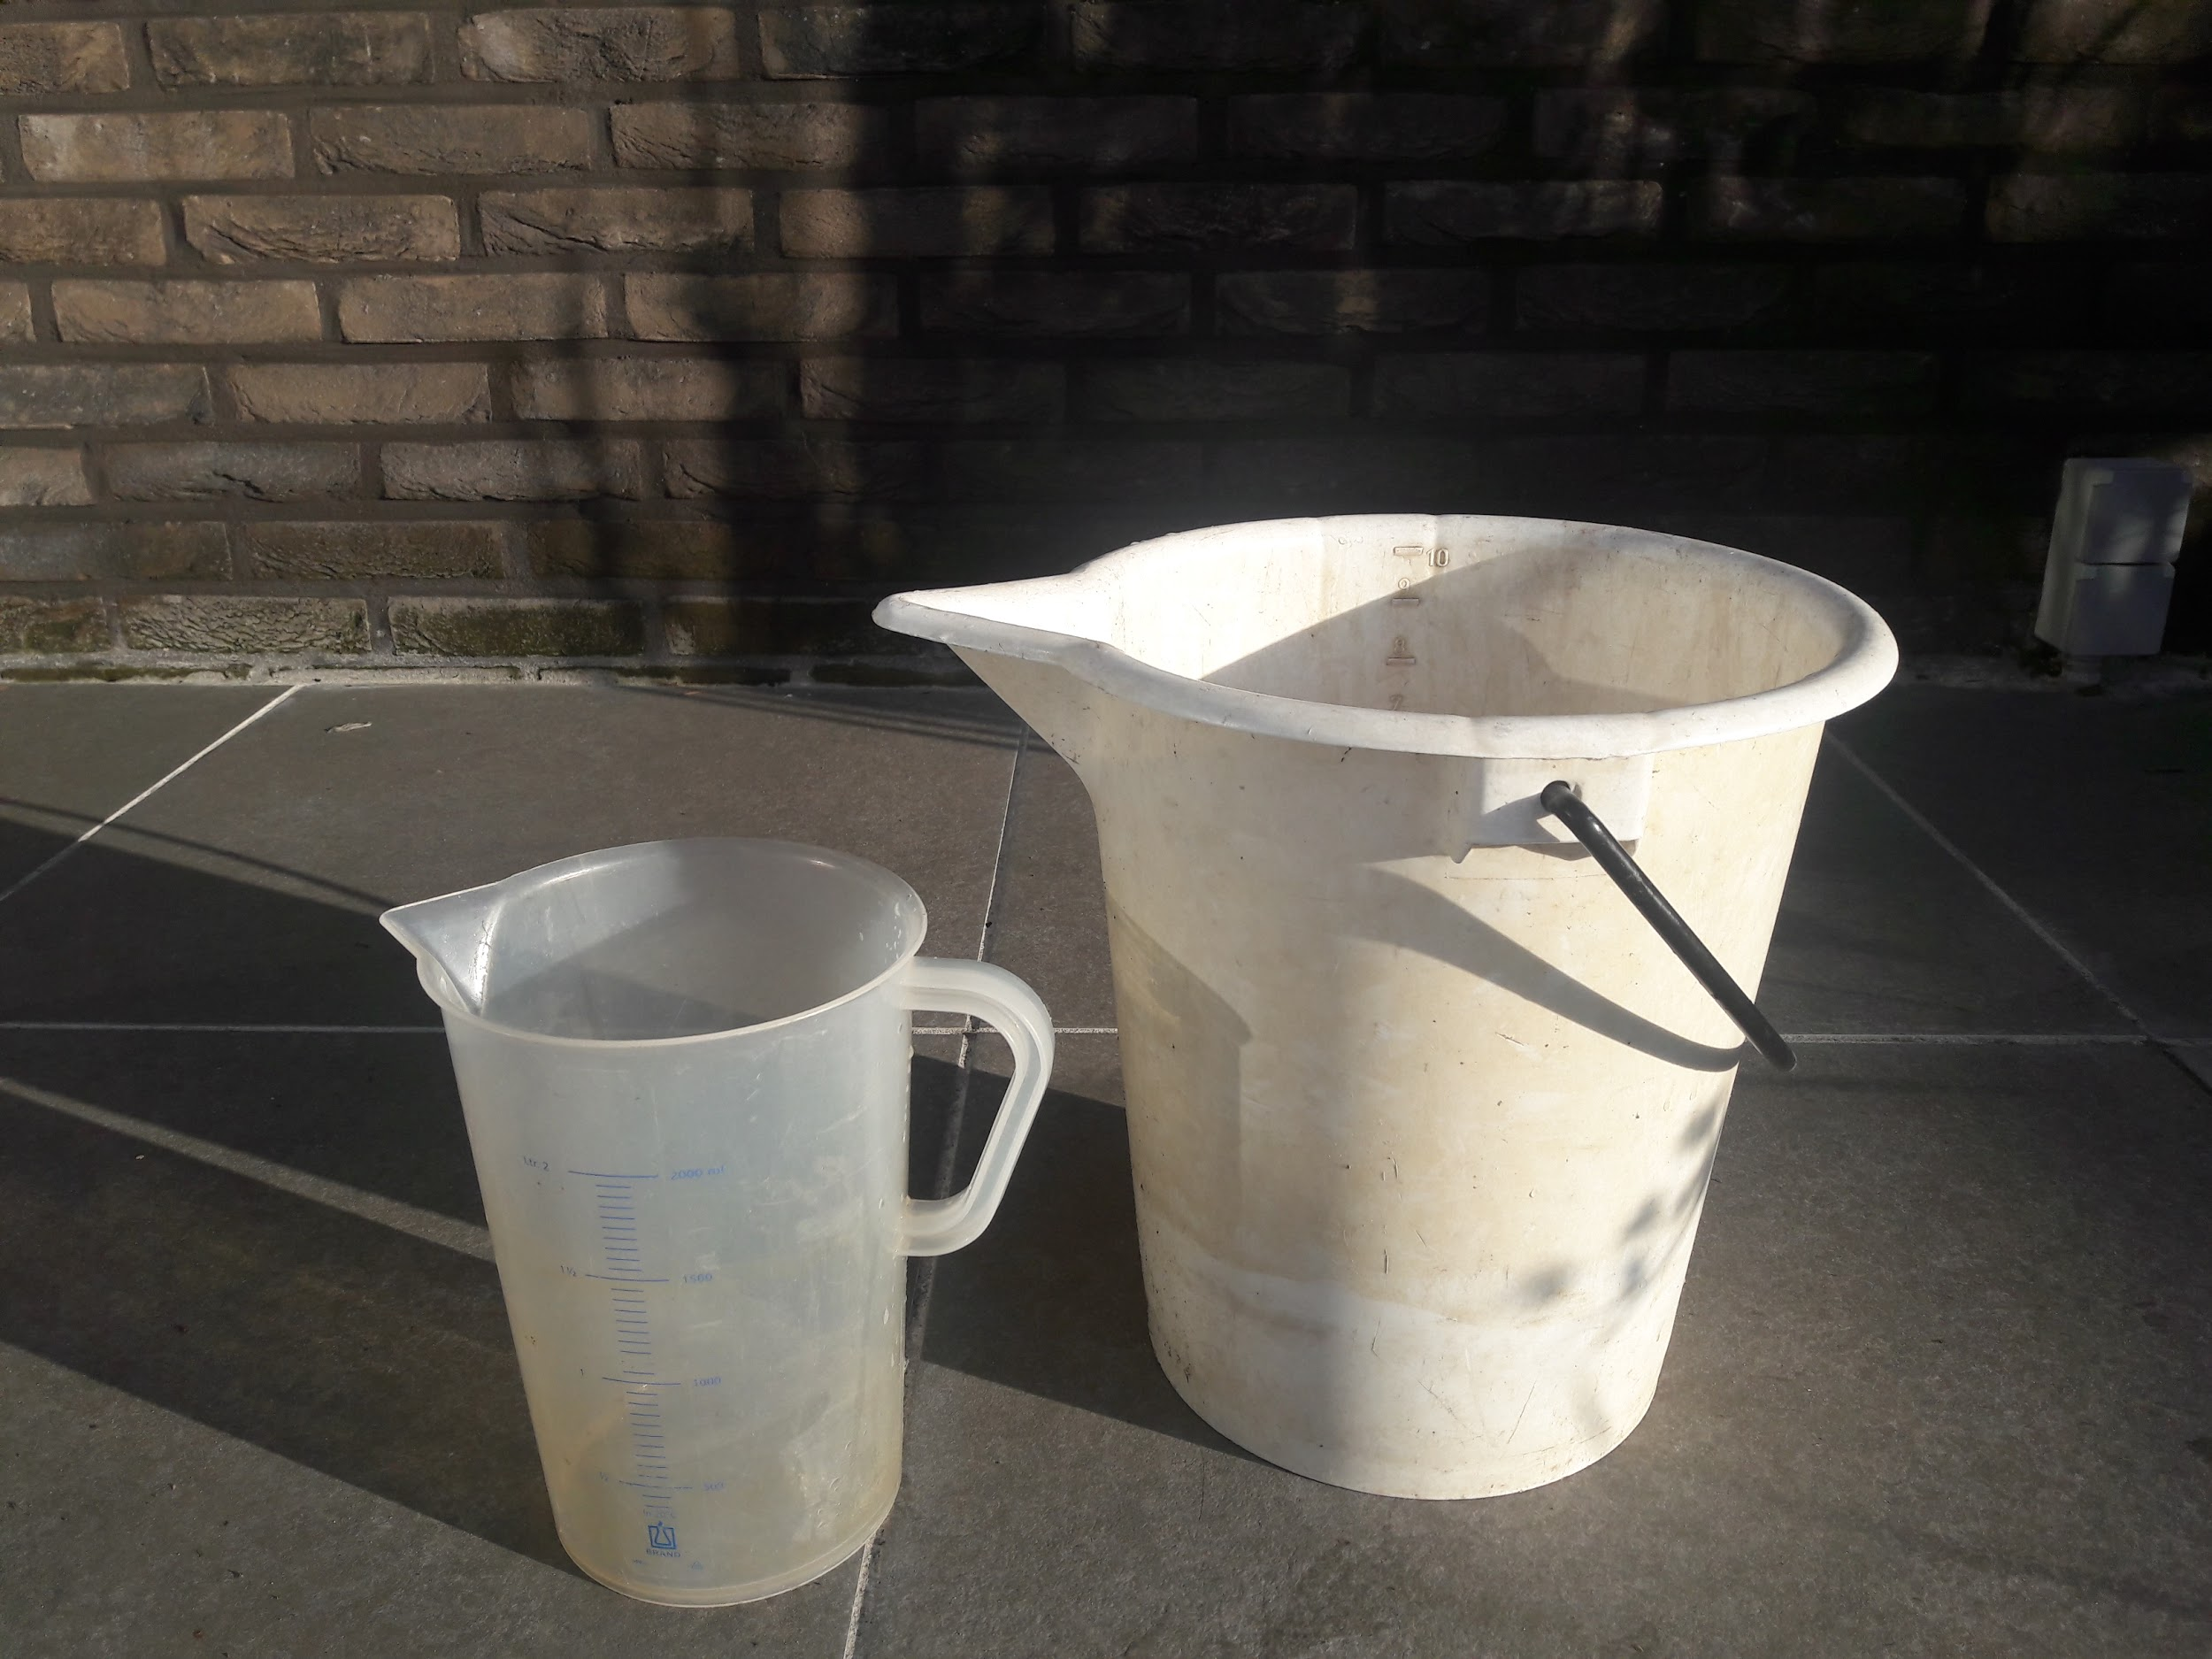
\includegraphics[width=6.29966in,height=4.72222in]{./media/image1.jpg}
\caption{Figuur 1: Maatbeker (links) en staalname-emmer (rechts).}
\end{figure}

\textbf{Recipiënten}

Voor elk staal zijn er, bij standaard staalname, zeven recipiënten voorzien (figuur 2). Elk recipiënt is voorzien van een label met een unieke code en een streepjescode per staal voor invoer in LIMS (= laboratory information management system). Ieder recipiënt dient voor een specifieke analyse (

tabel 2). Gebruik daarom steeds de correcte recipiënten (nummers refereren naar figuur 2):

\begin{itemize}
\item
  \textbf{1}, Fles 1.000 ml (\textbf{FL-1000R}, \textbf{FL-1000W}): vierkante fles van 1.000 ml met smalle hals en platte bodem, vervaardigd uit high density polyethyleen (HDPE), gegradueerd, met rode schroefdop.
\item
  \textbf{2 en 3}, Fles, 250 ml (\textbf{FL-250R}, \textbf{FL-250W}, \textbf{FL-250B}): vierkante fles van 250 ml met brede hals en platte bodem, vervaardigd uit high density polyethyleen (HDPE), gegradueerd, met blauwe, rode of witte schroefdop.
\item
  \textbf{4}, Fles, 100 ml (\textbf{FL-100R}) : vierkante fles van 100 ml met smalle hals en platte bodem, vervaardigd uit high density polyethyleen (HDPE), niet-gegradueerd, met rode schroefdop.
\item
  \textbf{5}, Falcontube, 50 ml (\textbf{FT-50B}, \textbf{FT-50R, FT-50G}): cilindrisch buisje of tube van 50 ml met conische bodem vervaardigd uit polypropyleen (PP), gegradueerd, met rode schroefdop vervaardigd uit polyethyleen (PE).
\item
  \textbf{6}, Falcontube, 50 ml (\textbf{FT-50B}, \textbf{FT-50R, FT-50G}): cilindrisch buisje of tube van 50 ml met conische bodem vervaardigd uit polypropyleen (PP), gegradueerd, met blauwe schroefdop vervaardigd uit polyethyleen (PE).
\item
  \textbf{7}, Falcontube, 30 ml (\textbf{FT-30W}): cilindrisch buisje of tube van 30 ml met conische bodem met rechtstaand stuk, vervaardigd uit polypropyleen (PP), niet-gegradueerd, met witte schroefdop vervaardigd uit polyethyleen (PE).
\end{itemize}

\begin{figure}
\centering
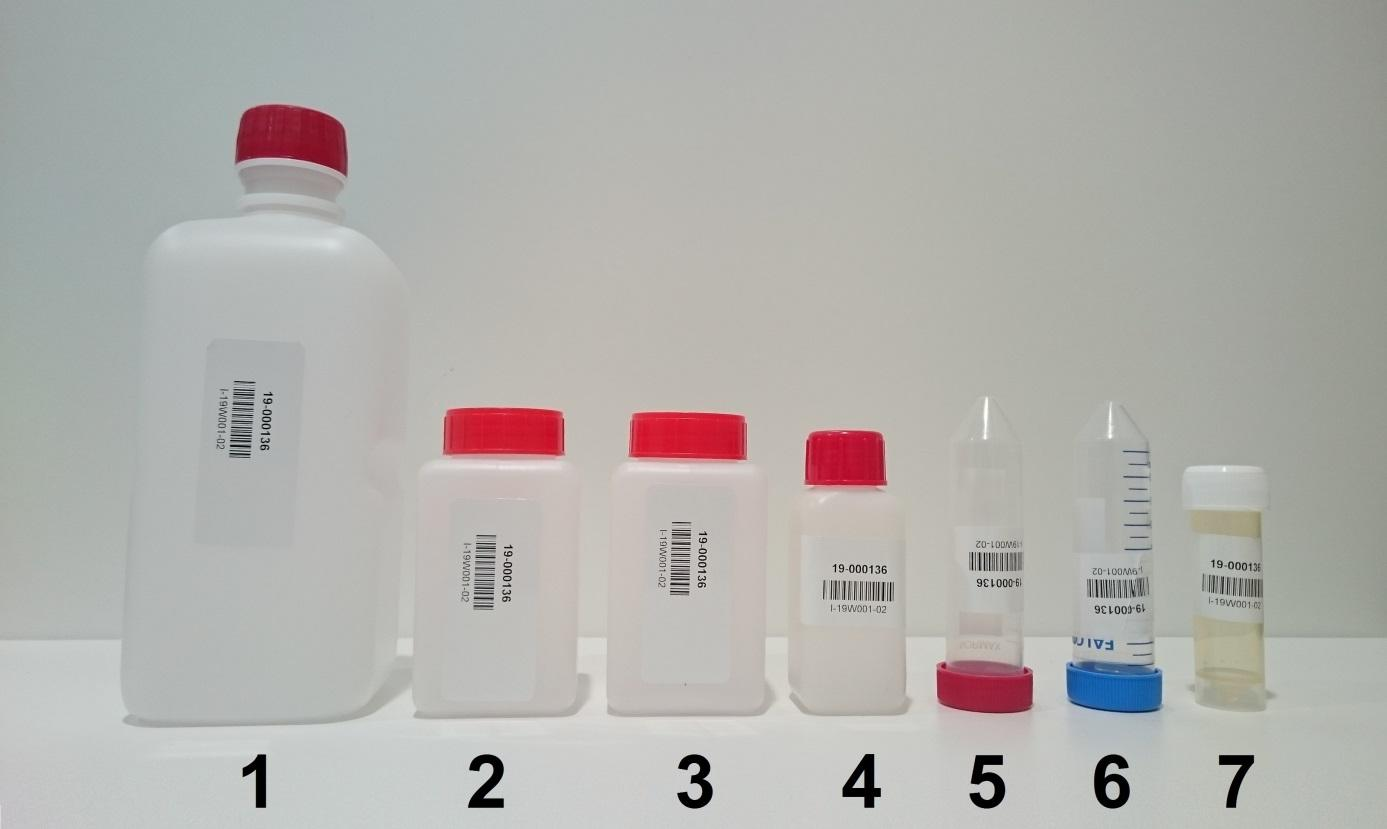
\includegraphics[width=6.29966in,height=3.76389in]{./media/image2.jpg}
\caption{Figuur 2: De 7 recipiënten die tijdens de staalname worden gevuld.}
\end{figure}

\begin{longtable}[]{@{}
  >{\raggedright\arraybackslash}p{(\columnwidth - 4\tabcolsep) * \real{0.2083}}
  >{\raggedright\arraybackslash}p{(\columnwidth - 4\tabcolsep) * \real{0.2083}}
  >{\raggedright\arraybackslash}p{(\columnwidth - 4\tabcolsep) * \real{0.5833}}@{}}
\toprule\noalign{}
\endhead
\bottomrule\noalign{}
\endlastfoot
\textbf{recipiënt} & \textbf{beschrijving} & \textbf{analyse} \\
1 & 1 l & zwevende stof \\
2 & 250 ml & chlorofyl \emph{a} \\
3 & 250 ml & bicarbonaatbepaling (TAP-TAM), IC (ionenuitwisselingschromatografie), controle pH en EC, kleur \\
4 & 100 ml & TP (totaalfosfor), KjN (Kjelldahl-stikstof), COD (chemisch zuurstofverbruik) \\
5 & Falcon 50 ml rode dop & reservestaal \\
6 & Falcon 50 ml blauwe dop & DOC (opgelost organisch koolstof) \\
7 & 30 ml met 300 µl salpeterzuur (1\%) & ICP (metalen) \\
\end{longtable}

Tabel 2: Analyses die uitgevoerd worden op de waterstalen van de respectievelijke recipiënten.

Houd de afzonderlijke recipiënten van eenzelfde staal steeds bijeen in de daarbij horende plastic zak met gripsluiting om te voorkomen dat recipiënten gecontamineerd worden tijdens het transport, verloren gaan of dat recipiënten van verschillende stalen door elkaar worden gehaald.

Ook dient steeds minstens één volledige set van reserverecipiënten voorhanden te zijn voor het geval een set recipiënten onvolledig is, gecontamineerd is (bijv. door het uitlopen van salpeterzuur uit recipiënt 7), of door enige andere reden onbruikbaar blijkt.

De recipiënten dienen voorafgaand aan de staalname volstrekt zuiver te worden gehouden. Elk contact met de binnenzijde van de recipiënten en hun deksels dient te worden vermeden.

\textbf{Spuiten en filters}

Het recipiënt met salpeterzuur (recipiënt nummer 7) dient te worden gevuld met gefilterd water. De filtratie gebeurt in het veld door de gevulde spuit te voorzien van een opzetfilter en de spuit voorzichtig te ledigen in het recipiënt. Hiervoor worden spuiten van 35 ml met een conus met Luer-lock (schroefdraad in de conus) en A-20/25 filters met een membraan met poriëngrootte van 0,20 µm gebruikt (figuur 3). De filter wordt met de klok mee vastgedraaid in de conus. Om contaminatie te vermijden worden de filters slechts eenmaal gebruikt. Meerdere filters kunnen nodig zijn voor het filteren van 25 tot 30 ml, de hoeveelheid water nodig om een ICP-analyse te kunnen uitvoeren. De filter wordt vervangen wanneer het water er met veel druk slechts traag uit druppelt. De spuiten kunnen voor meerdere staalnamepunten worden herbruikt, maar moeten dan steeds voorgespoeld worden met waterstaal, dit door de spuit minstens drie maal te vullen en vervolgens terug leeg te spuiten. De spuiten worden steeds vervangen tussen sterk verschillende oppervlaktewateren en worden niet langer dan één dag gebruikt. Bewaar ongebruikte filters steeds in een schoon, droog en goed afgesloten zakje of ander recipiënt om contaminatie te voorkomen.

\begin{figure}
\centering
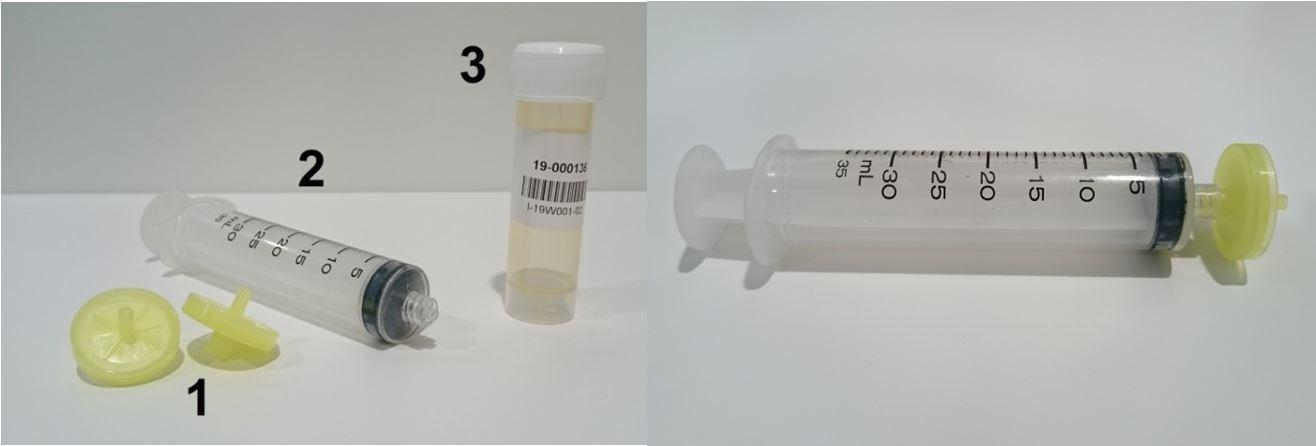
\includegraphics[width=6.29966in,height=2.13889in]{./media/image3.jpg}
\caption{Figuur 3: Links: filters (A-20/25) met een membraan met poriëngrootte van 0,20 µm (1) en spuiten (35 ml) met een conus met Luer-lock (2) en recipiënt met salpeterzuur 65\% (3) Rechts: spuit met vastgeschroefde filter.}
\end{figure}

\textbf{Staalnameformulier (analoog of digitaal):}

Het staalnameformulier (zie SPP-116 bijlage 1) kan zowel digitaal als analoog ingevuld worden in het veld. Bij voorkeur wordt tijdens de staalname steeds de analoge versie ingevuld zodat typfouten of problemen bij gegevensopslag worden vermeden en er tevens een originele versie beschikbaar is voor controle op een later tijdstip. Het staalnameformulier wordt duidelijk leesbaar en volledig ingevuld met potlood, dat in tegenstelling tot inkt ook schrijft in natte omstandigheden en niet kan uitlopen.

\textbf{Koelbox en koelelementen}

Een ruime, dubbelwandige en goed afsluitende koelbox en ingevroren koelelementen zijn nodig om de stalen tijdens de veldwerkzaamheden en transport goed te kunnen conserveren. De koelelementen mogen geen defecten (lekkage) vertonen. De koelelementen en de koelbox zijn bij voorkeur gemakkelijk te reinigen om contaminatie van de stalen te voorkomen.

\section{Reagentia en oplossingen (indien van toepassing)}\label{reagentia-en-oplossingen-indien-van-toepassing}

\textbf{Salpeterzuur 65\%, suprapur, (HNO\textsubscript{3}):} Sterk zuur dat zowel irriterend en corrosief werkt. Draag handschoenen bij gebruik, voorkom inademing van dampen en contact met de huid en ogen.

\chapter{Werkwijze}\label{werkwijze}

\section{Uitvoering}\label{uitvoering}

Hieronder wordt puntsgewijs een gedetailleerde omschrijving gegeven van alle stappen die doorlopen moeten worden om het veldprotocol uit te voeren.

\subsection{\texorpdfstring{\textbf{Vastleggen toestand staalnamepunt}}{Vastleggen toestand staalnamepunt}}\label{vastleggen-toestand-staalnamepunt}

Eerst wordt de toestand van het staalnamepunt gedocumenteerd op het staalnameformulier, waarbij uitzonderlijke waterstanden of weersomstandigheden, potentiële contaminanten (zoals opwarrelend slib, aanwezigheid van zoöplankton in het staal) of factoren die de correcte uitvoering van de procedure bemoeilijken (zoals ijs of een kroosdek) worden genoteerd (zie ook 2.3). Zo kan je hiermee rekening houden bij de staalname. Neem bij elke staalname en/of veldmeting steeds een overzichtsfoto en eventueel detailfoto's zodat dit later kan worden geraadpleegd.

\subsection{\texorpdfstring{\textbf{Voorbereiding}}{Voorbereiding}}\label{voorbereiding}

Bij aanvang van het veldwerk wordt het materiaal dat in contact komt met het staal overvloedig gespoeld met water van de staalnamelocatie. Spoelen met lokaal water helpt het materiaal te acclimatiseren aan het staal en beperkt de residuen van producten of vorige stalen. Doe dit zowel voor de recipiënten (uitgez. recipiënt nummer 7), staalname-emmer, maatbeker, spuit, latex handschoenen en laarzen als voor de elektrodes van de multimeter. Indien recipiënten gecertificeerd zijn als `contaminant-vrij' is het spoelen van de recipiënten niet noodzakelijk.

\subsection{\texorpdfstring{\textbf{Nemen van een mengstaal}}{Nemen van een mengstaal}}\label{nemen-van-een-mengstaal}

Kies eerst een geschikte plaats voor de staalname, op of in de directe omgeving (zo dicht mogelijk) van het staalnamepunt. Neem geen (deel)staal op plekken die recent werden verstoord door dieren of mensen. Ganzen, vee, etc. kunnen door verstoring van de waterbodem en de vegetatie, of door hun fecaliën, of het inbrengen van locatievreemd materiaal het staal contamineren. Neem indien mogelijk geen (deel)staal tussen dichte vegetatie en hou voldoende afstand van in- en uitstroompunten van waterlopen, duikers of lozingsvoorzieningen, tenzij dit specifiek wenselijk is. Wees alert voor plaatselijke contaminanten bij locaties naast wegen (bijvoorbeeld afstroom van regenwater van weginfrastructuur, strooizout in de winter, etc.) en andere antropogene elementen.

Maak een mengstaal door met de maatbeker op drie punten (bij voorkeur twee of drie meter uit elkaar) een gelijk volume deelstaal (twee liter) te nemen. Doe dit steeds voorzichtig zonder de waterbodem of vegetatie te veel te verstoren. Laat de maatbeker diep genoeg zakken zodat het deelstaal water van de waterkolom bevat en niet enkel het water aan het oppervlak. Giet de inhoud van de maatbeker voorzichtig in de staalname-emmer zonder luchtbellen te veroorzaken.

Indien het nemen van een staal gehinderd wordt door ijsvorming wordt eerst een voldoende grote opening in het ijs gemaakt waaruit alle brokken ijs en eventueel vuil en slib worden verwijderd. Vervolgens wacht men enkele minuten zodat het water vrij onder het ijs kan bewegen. Om contaminatie van omgewoelde bodem te vermijden wordt enkel bemonsterd als er minstens circa 10 cm water aanwezig is onder de ijslaag (VMM 2020). Deze werkwijze mag enkel uitgevoerd worden wanneer de veiligheid van de staalnemer gegarandeerd kan worden.

\subsection{\texorpdfstring{\textbf{Vullen van recipiënten voor het laboratorium}}{Vullen van recipiënten voor het laboratorium}}\label{vullen-van-recipiuxebnten-voor-het-laboratorium}

\begin{enumerate}
\def\labelenumi{\arabic{enumi}.}
\tightlist
\item
  \ul{\emph{Vul het recipiënt voor IPC met spuit en filters}}
\end{enumerate}

Na het nemen van het mengstaal wordt eerst de spuit gevuld (de analyses op het staal van dit recipiënt zijn het meest contaminatiegevoelig). Spoel de spuit voor met staal en vul deze opnieuw (3 x). Draai de filter vast op de spuit (met de klok mee) en vul recipiënt 7 (Falcontube 30 ml met salpeterzuur 65\%). Wanneer het water slechts traag door de filter druppelt, wordt een nieuwe filter gebruikt. Het recipiënt wordt met minstens 25 ml staal gevuld omdat de hoeveelheid salpeterzuur (1\%) in het recipiënt op deze hoeveelheid staal is afgestemd. \textbf{Wees steeds voorzichtig bij het gebruik van salpeterzuur, draag handschoenen, voorkom inhalatie van dampen en contact met de huid en ogen.}

\begin{enumerate}
\def\labelenumi{\arabic{enumi}.}
\setcounter{enumi}{1}
\tightlist
\item
  \ul{Vul de overige recipiënten}
\end{enumerate}

Vul nu de overige recipiënten in de aangegeven volgorde, startend met recipiënt 6 en eindigend met recipiënt 1 (zie tabel 2). De volgorde stemt overeen met de gevoeligheid van de analyses die per recipiënt worden uitgevoerd, waarbij de meest contaminatiegevoelige eerst worden gevuld. Doe dit voorzichtig en beperk de aanwezigheid van luchtbellen tot een minimum. Vul de recipiënten altijd tot aan de rand. Het vermijden of beperken van extra zuurstof in een waterstaal is een beperkende factor voor chemische en (micro-)biologische reacties welke de kwaliteit van het staal negatief kunnen beïnvloeden.

Bij het openen van de recipiënten mogen de doppen niet met de onderkant (binnenzijde) op de ondergrond worden geplaatst. Leg open recipiënten niet op de grond, maar zet deze steeds recht op een stabiel oppervlak. De recipiënten worden net voor het vullen geopend en onmiddellijk na het vullen gesloten om de kans op contaminatie te minimaliseren.

De 7 gevulde recipiënten worden steeds per staalnamepunt bijeen gevoegd in een zakje met gripsluiting. Ze worden koel (max. 4 °C) en donker bewaard in een goed afsluitende, koelbox met koude koelelementen. Bij lagere temperaturen wordt de microbiologische activiteit van de micro-organismen en chemische reacties vertraagd en blijft de toestand van het staal langer stabiel. Voor verdere richtlijnen rond het bewaren van waterstalen in het veld en tijdens transport wordt verwezen naar het protocol SOP-005.

\subsection{\texorpdfstring{\textbf{Schoonmaken materiaal}}{Schoonmaken materiaal}}\label{schoonmaken-materiaal}

Na de staalname wordt het materiaal (emmer, maatbeker en spuit) ter plaatse gespoeld met overvloedig lokaal water om contaminatie met substraat of organismen op de volgende locatie te beperken.

\section{Registratie en bewaring van resultaten}\label{registratie-en-bewaring-van-resultaten}

De stalen worden zo snel mogelijk (binnen 24 uur na het nemen van het eerste staal) binnengebracht bij het analytisch labo. In het analytisch labo worden de stalen, in afwachting van verdere analyse, in de koelkamer bewaard.

Bij de levering van de stalen aan het laboratorium wordt steeds een kopie gemaakt van het ingevulde staalnameformulier en samen met de stalen overhandigd. Het originele formulier wordt bewaard door de projectverantwoordelijke. Het staalnameformulier wordt vervolgens door de staalnemer gedigitaliseerd door de gegevens van het staalnameformulier manueel in te voeren in het digitale staalnameformulier op Google Drive.

\chapter{Kwaliteitszorg}\label{kwaliteitszorg}

De kwaliteit van het analyseresultaat wordt in belangrijke mate bepaald door de representativiteit van het staal. Kwaliteitszorg bij het nemen hiervan is dus een belangrijk gegeven. Ongebruikte recipiënten dienen steeds gesloten te worden bewaard in een droge en stofvrije ruimte. Het hergebruik van recipiënten is niet toegestaan omdat residu's van voorgaand gebruik het staal kunnen beïnvloeden. Onderhoud en het grondig reinigen van het staalnamemateriaal zijn van groot belang in het voorkomen van contaminatie en worden voorzichtig en correct uitgevoerd. Alleen correct gereinigd materiaal mag getransporteerd en gebruikt worden in het veld. De handen van de staalnemer moeten proper zijn en er worden latex handschoenen (poederloos) gebruikt. Bij aanvang van de staalname, dient het materiaal dat in contact komt met het staal grondig gespoeld te worden met water van de staalnamelocatie en in geen geval gereinigd met detergenten etc., omdat deze het staal kunnen contamineren. Spoelen met lokaal water helpt tevens het materiaal te acclimatiseren aan het staal en beperkt de contaminatie van producten of vorige stalen. Indien recipiënten werden gecertificeerd als `contaminant-vrij' is het spoelen van de recipiënten niet noodzakelijk.

Het is van groot belang om bij het waden zeer voorzichtig te werk te gaan om vertroebeling tot een minimum te beperken en eventueel te wachten tot alles terug bezonken is.

De omgevingsfactoren die invloed kunnen hebben op de kwaliteit van het staal (zie 2.3 Beperkingen tot de procedure) worden op het staalnameformulier in het opmerkingenveld ingevuld. Deze worden in een databank ingevoerd.

Het waterstaal kan veranderingen ondergaan ten gevolge van chemische en biologische processen. Om dit tegen te gaan is het belangrijk om de hoeveelheid zuurstof in de recipiënten bij de staalname te beperken en de stalen nadien koel en donker te bewaren. Bij de laboratoriumanalyses van de stalen wordt steeds de zuurtegraad en conductiviteit opnieuw gemeten ter controle en vergeleken met de veldmetingen om eventuele afwijkingen te signaleren.

\chapter{Veiligheid}\label{veiligheid}

Om mogelijke besmetting en verwondingen bij de staalnemer en mogelijke contaminatie van het staal te voorkomen, worden tijdens de waterstaalname waterbestendige, poederloze handschoenen gedragen.

Draag bij het werken met salpeterzuur (recipiënt 7) steeds handschoenen, voorkom contact met de huid en ogen en adem de dampen niet in. Contact met de huid kan een tijdelijke (enkele dagen) verkleuring veroorzaken.

Alle algemene veiligheidsregels voor het werken in en langs water of vanuit een boot zijn van toepassing (zie protocol Veiligheid in en rond water SVP-112).

Ook bioveiligheidsmaatregelen in verband met de verspreiding van organismen tussen oppervlaktewateren, inz. invasieve niet-inheemse soorten en pathogenen, zijn van toepassing (zie protocol Bioveiligheidsmaatregelen SVP-015).

\chapter{Samenvatting}\label{samenvatting}

Een samenvattende opsomming van de te volgen stappen:

\begin{enumerate}
\def\labelenumi{\arabic{enumi}.}
\item
  spoel het materiaal voor met water van het staalnamepunt;
\item
  neem een mengstaal (bestaande uit drie tot vijf deelstalen te nemen met de maatbeker);
\item
  vullen van recipiënten voor het laboratorium:

  \begin{enumerate}
  \def\labelenumii{\arabic{enumii}.}
  \item
    vul het recipiënt 7 voor IPC met spuit en filters;
  \item
    vul nadien de overige recipiënten (startend met recipiënt 6 en eindigend met recipiënt 1);
  \end{enumerate}
\item
  steek de gevulde recipiënten per staalnamepunt samen in een zakje met gripsluiting en bewaar deze in de koelbox;
\item
  reinig het gebruikte materiaal;
\item
  breng de stalen en een kopie van het staalnameformulier binnen bij het labo (binnen 24u na het nemen van het eerste staal);
\item
  digitaliseer het staalnameformulier en klasseer de foto's (registratie).
\end{enumerate}

\chapter{Referenties}\label{referenties}

Canfield D.E., Shireman J.V., Colle D.E., Haller W.T., Watkins C.E., \& Maceina M. J., 1984. Prediction of chlorophyll \emph{a} concentrations in Florida lakes: Importance of aquatic macrophytes. Canadian Journal of Fisheries and Aquatic Sciences,41(3), 497--501. \url{https://doi.org/10.1139/f84-059}

DIW (2003). Decreet Integraal Waterbeleid van 18 juli 2003 (B.S. 5/12/2003). \href{https://navigator.emis.vito.be/mijn-navigator?woId=75697}{\ul{https://navigator.emis.vito.be/mijn-navigator?woId=75697}}

VMM (2020). Procedure voor de monsterneming en verdeling van oppervlaktewater t.b.v. fysisch-chemisch onderzoek d.m.v. een schepmonster. VMM/WAT/GP/3.105; uitgave 15. Vlaamse Milieumaatschappij, Aalst.

\chapter{(APPENDIX) Bijlagen}\label{appendix-bijlagen}

n.v.t.

\end{document}
